\section{Detection Method (G1)}\label{sec:method}
Fig.~\ref{fig:pipeline} shows the pipeline. Meters whose readings for two consecutive intervals have
not arrived form a \emph{silent group} with a common onset $t_0$. At a decision time $\tau$, using only
data that had arrived by $\tau$, the method computes over the window $w=[t_0,\tau)$
\begin{align}
R &= \textstyle\sum_{t\in w}\big(T_t - \sum_{m\in K_t} E_{m,t} - g_0 - \hat{O}_t\big), \label{eq:R}\\
M &= \textstyle\sum_{t\in w}\sum_{m\in G}\big(\bar{E}_{m,t} + \rho_{\ell}\,\delta_{m}\big), \label{eq:M}
\end{align}
where $T_t$ is the transformer's LV energy in interval $t$, $K_t$ the meters whose reading for $t$
has arrived, $E_{m,t}$ their energy, $g_0$ the median transformer-to-meters gap over the last day,
$\hat{O}_t$ the expected energy of other missing meters, $G$ the silent group, $\bar{E}_{m,t}$ the mean
of the same 15-min slot over the previous 14 days, $\delta_m$ the deviation of meter $m$ from that
mean just before the onset, and $\rho_\ell$ a persistence factor fitted per lead $\ell$. All energies
are in kWh. If the customers still have power, $R \approx M$; if they lost it, $R \approx 0$.

\begin{figure*}[!t]
\centering
% System pipeline (illustration). Every element is named in the paper text (Sections V to VIII).
\begin{tikzpicture}[
  font=\footnotesize, node distance=4mm and 3.2mm,
  box/.style={draw, rounded corners=1.5pt, align=center, inner sep=3pt, minimum height=11mm, text width=#1},
  box/.default=21mm,
  prop/.style={box=#1, dashed, fill=gray!8},
  prop/.default=21mm,
  arr/.style={-{Stealth[length=2mm]}, semithick}]
\node[box=20mm] (meters) {Smart meters and the transformer meter};
\node[box=22mm, right=of meters] (obs) {Observed data with arrival times (+ static context)};
\node[box=21mm, right=of obs, yshift=7.5mm, minimum height=9mm] (cons) {Learned consumption model};
\node[box=21mm, right=of obs, yshift=-7.5mm, minimum height=9mm] (noise) {Learned noise model};
\node[box=24mm, right=of obs, xshift=26mm] (reason) {Probabilistic reasoning: outage vs communication failure};
\node[box=25mm, right=of reason] (sel) {Selective prediction: OUTAGE / COMMUNICATION FAILURE / UNCERTAIN};
\node[box=19mm, below=5mm of sel] (esc) {Escalation table};
\node[box=19mm, left=of esc] (op) {Operator console (preview)};
\node[box=22mm, left=of op] (log) {Hash-chained decision log};
\node[prop=26mm, left=8mm of log] (share) {Shared learning between nodes (PROPOSED; proof of concept measured)};
\draw[arr] (meters) -- (obs);
\draw[arr] (obs.east) -- ++(1.5mm,0) |- (cons.west);
\draw[arr] (obs.east) -- ++(1.5mm,0) |- (noise.west);
\draw[arr] (cons.east) -- ++(1.5mm,0) |- (reason.west);
\draw[arr] (noise.east) -- ++(1.5mm,0) |- (reason.west);
\draw[arr] (reason) -- (sel);
\draw[arr] (sel) -- (esc);
\draw[arr] (esc) -- (op);
\draw[arr] (op) -- (log);
\draw[arr, dashed] (log) -- (share);  % confirmed outcomes with their evidence numbers (Section 5.4)
\end{tikzpicture}

\caption{System pipeline. Solid boxes are IMPLEMENTED and evaluated in simulation; dashed boxes are
PROPOSED. The meter-count gate and the re-check of Section~\ref{sec:governance} are evaluated in study
code and are not yet executed by the escalation step.}\label{fig:pipeline}
\end{figure*}

\textbf{Decision.} With Student-t likelihoods of 4 degrees of freedom, scales $s_O$ (outage) and
$s_C$ (communication failure) built from the fitted gap noise and forecast spread, and a prior of
one half for each cause, the posterior probability of a communication failure is
\begin{equation}
p = \sigma\!\left(\ln f_\nu\!\left(\tfrac{R-M}{s_C}\right) - \ln s_C - \ln f_\nu\!\left(\tfrac{R}{s_O}\right) + \ln s_O\right), \label{eq:p}
\end{equation}
where $f_\nu$ is the Student-t density and $\sigma$ the logistic function. The verdict is
COMMUNICATION FAILURE if $p \ge 1-b$, OUTAGE if $p \le b$, and UNCERTAIN otherwise, with abstention
band $b = 0.03$. The decision is taken at the first of up to five decision times at which it is not
UNCERTAIN.

\textbf{Fitting and threshold selection.} Noise and persistence parameters are fitted on each
network's own fault-free history (training weeks); no labelled data is needed. The band $b$ was chosen
once, on development validation weeks, as the setting that abstains least while keeping missed
outages at or below 0.05, false outages at or below 0.05 and fault-free false outages at or below
0.001 per meter-day (DESIGN CHOICE). Two earlier selection rules failed and are reported in the
repository: one called 419 of 1051 fault-free silent groups outages, the other missed 0.366 of outages.

\textbf{Why not a trained classifier.} Under the same safety limits, logistic regression, gradient
boosting and a small neural network trained on simulated labels missed 0.089, 0.179--0.196 and
0.232--0.250 of validation outages, against 0.036 for the fitted method; none had a feasible
abstention band (Fig.~\ref{fig:classifiers}). The fitted probabilistic parameters are therefore the
trained models of this submission, by a measured choice.

\begin{figure}[!t]
\centering
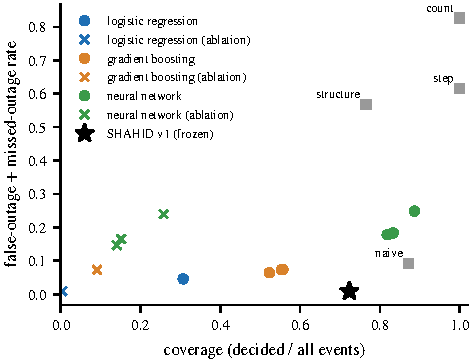
\includegraphics[width=\columnwidth]{figures/classifier_coverage_safety.pdf}
\caption{Coverage against false-outage plus missed-outage rate on the held-out urban network, test
weeks (SIMULATED, post-hoc). Dots: classifiers, one per seed; crosses: without energy-balance
features; squares: simple baselines; star: the frozen method.}\label{fig:classifiers}
\end{figure}

\subsection{Scope boundary: single-meter anomalies}\label{sec:singlemeter}
Silent groups were chosen first because the same symptom needs opposite responses and the
transformer gives an independent physical witness. Faults inside one meter that keeps reporting
(gain, bias, noise) are a different problem: the balance can show that some meter is
wrong, not which one. We tested them. Injected gain errors, biases and noise on one meter were
detected in at most 20\% of cases; a per-meter regression of the transformer gap detected a gain of
0.5 in 0.347 of cases on a network never used before, and neighbour-voltage comparison detected at
most 0.053. Single-meter fault detection is therefore outside the validated scope. The Phase 2 path
(PROPOSED, not implemented): residual drift tracked per meter over weeks, comparison with electrically
adjacent meters with field voltage data, and escalation to human review instead of automatic action.
